\chapter{Docker}

\section{Opis rozwiązania Docker}

Docker jest narzędziem ułatwiającym proces tworzenia, dystrybucji i wdrażania oprogramowania. Pozwala on na umieszczenie aplikacji wraz z jej bezpośrednimi zależnościami w kontenerze i uruchomienie jej na dowolnej maszynie z systemem Linux. Aplikacje działające za pomocą Dockera są odizolowane od infrastruktury, dzięki czemu możliwe jest uruchomienie kilku niezależnych kontenerów z aplikacjami symulujących pracę w środowisku rozproszonym. Jednocześnie narzędzie to zapewnia niewielkie zużycie pamięci dzięki współdzieleniu warstw UFS obrazów (ang. Union File System) pomiędzy kontenerami. Współdzielenie jądra systemu pomiędzy kontenerami, a systemem gospodarza zapewnia natomiast krótkie czasy uruchomienia. Ze względu na te cechy korzystanie z aplikacji uruchomionej za pomocą Dockera jest niemal tak wydajne, jak działającej na systemie gospodarza.

	Podstawowymi komponentami Dockera są:
\begin{itemize}
\item \textit{Docker Engine} -  platforma do tworzenia kontenerów na uruchamiane przez użytkownika aplikacje,
\item \textit{Docker Hub} – oficjalne repozytorium obrazów przechowujące obrazy udostępniane przez użytkowników
\end{itemize}

	Docker działa w architekturze klient – serwer. Do komunikacji klienta z demonem wykorzystywany jest protokół HTTP i odbywa się ona poprzez gniazda (ang. sockets) lub RESTful API. Klient Dockera jest podstawowym interfejsem komunikacyjnym z Dockerem – przyjmuje komendy z określonego zestawu poleceń wpisywane przez użytkownika i przekazuje je do demona. Demon odpowiada za budowanie obrazów, uruchamianie i dystrybucję kontenerów. Klient i demon mogą działać na tym samym systemie lub ich funkcje mogą zosać rozdzielone pomiędzy różne hosty.

Podstawowymi pojęciami Dockera są:
\begin{itemize}
\item \textit{obrazy} – komponent  odpowiadający budowaniu,
\item \textit{rejestry} – komponent odpowiadający dystrybucji,
\item \textit{kontenery} – komponent odpowiadający uruchamianiu.
\end{itemize}

	\textbf{\underline{Obraz}} jest to szablon służący tylko do odczytu, stanowiący podstawę do utworzenia kontenera. Obraz może zawierać np. system operacyjny Ubuntu z serwerem Apache oraz zainstalowaną aplikacją webową, którą chcemy uruchomić. Za pomocą Dockera mamy możliwość budowania nowych obrazów, aktualizowania istniejących, pobierania obrazów stworzonych przez innych i udostępniania własnych. Każdy obraz składa się z warstw tworzących ujednolicony system plików (\textit{ang. UFS}).  Ta technologia powoduje, że obrazy Dockera są lekkie – wprowadzenie zmian w aplikacji nie wiąże się z przebudową całego obrazu, a jedynie z aktualizacją lub dodaniem danej warstwy.
	
	Każdy obraz ma obraz bazowy (np. obraz systemu Ubuntu lub obraz utworzony przez użytkownika), na podstawie którego jest budowany za pomocą zestawu instrukcji. Każda instrukcja powoduje dodanie warstwy do naszego obrazu (taką instrukcją może być np. wywołanie komendy, dodanie pliku lub folderu, instalacja pakietu, utworzenie zmiennej środowiskowej). Polecenia tworzące obraz Dockera przechowywane są w pliku Dockerfile. Podczas budowania obrazu Docker odczytuje kod żródłowy zawarty w pliku Dockerfile, wykonuje zapisane instrukcje i zwraca końcowy obraz.

Przykładowe operacje na obrazie:
\begin{itemize}
\item Pobieranie obrazu:
\begin{lstlisting}[style=incode]
docker pull {nazwa obrazu}
\end{lstlisting}
\item Wyświetlanie lokalnie dostępnych obrazów:
\begin{lstlisting}[style=incode]
docker images
\end{lstlisting}
\item Wyświetlenie warstw składających się na obraz:
\begin{lstlisting}[style=incode]
docker history {id lub nazwa obrazu}
\end{lstlisting}
\item Usunięcie obrazu
\begin{lstlisting}[style=incode]
docker  rmi {id lub nazwa obrazu}
\end{lstlisting}
	
\end{itemize}

	\textbf{\underline{Rejestry}} są miejscem gdzie można udostępniać i skąd można pobierać obrazy. Mogą one być zarówno publiczne, jak i prywatne.  Publiczny rejestr Dockera stanowi Docker Hub zawierający bazę obrazów stworzonych przez użytkowników Dockera. Istnieje również lokalne repozytorium na maszynie użytkownika. Za pomocą klienta Dockera możliwe jest przeszukiwanie opublikowanych obrazów oraz pobieranie ich w celu utworzenia kontenera. 
	
	\textbf{\underline{Kontener}} tworzony jest na podstawie obrazu, który zawiera informacje o tym, co przechowuje kontener, jaki proces ma zostać uruchomiony po jego utworzeniu oraz inne dane konfiguracyjne. Kontener składa się z zestawu ujednoliconych warstw tylko do odczytu, pochodzących z obrazu kontenera oraz z pojedynczej warstwy do odczytu i zapisu umożliwiającej działanie procesów uruchamianych w kontenerze. Na kontenerach można wykonywać podstawowe operacje: uruchomić, zatrzymać, przenieść i usunąć.

Przykładowe operacje na kontenerze
\begin{itemize}
\item Tworzenie i uruchamianie kontenera:
\begin{lstlisting}[style=incode]
docker runl {nazwa lub id obrazu}
\end{lstlisting}
Uruchomienie tego polecenia z parametrem -d powoduje uruchomienie kontenera działającego w tle, natomiast parametr –rm=true powoduje, że kontener zostanie usunięty natychmiast po wykonaniu zadania.
\item Wyświetlanie wszystkich kontenerów:
\begin{lstlisting}[style=incode]
docker ps -a
\end{lstlisting}
\item Zatrzymanie kontenera
\begin{lstlisting}[style=incode]
docker stop {id lub nazwa kontenera}
\end{lstlisting}
\item Usunięcie kontenera
\begin{lstlisting}[style=incode]
docker rm {id lub nazwa kontenera}
\end{lstlisting}
\end{itemize}

	Docker udostępnia również możliwość automatycznego budowania obrazu w synchronizacji z systemem kontroli wersji (GitHub lub Bitbucket). Dzięki umieszczeniu w repozytorium pliku \textit{Dockerfile} oraz powiązaniu konta DockerHub I kontem w wybranym systemie kontroli wersji, po każdorazowej aktualizacji kodu w repozytorium budowany, na jego podstawie budowany jest aktualny obraz Dockera i zapisywany w repozytorium DockerHub.
	
	
	
	
\section{Raport z przykładowych uruchomień}

\subsection{Uruchomienie aplikacji \textit{'Hello World'}}
Aplikacja uruchamiana jest poleceniem
\begin{lstlisting}[style=incode]
$ docker run ubuntu /bin/echo 'Hello world'
\end{lstlisting}
gdzie:
\begin{itemize}
\item \textit{docker run} – uruchamia kontener
\item \textit{ubuntu} – obraz, na podstawie którego tworzony jest kontener (obraz systemu ubuntu)
\item \textit{/bin/echo  'Hello world'} – polecenie, które ma zostać wywołane wewnątrz 	utworzonego kontenera \newline
\end{itemize}
Odpowiedź Dockera na zadaną komendę:
\begin{lstlisting}[style=incode]
Unable to find image 'ubuntu:latest' locally
latest: Pulling from library/ubuntu
759d6771041e: Pull complete
8836b825667b: Pull complete
c2f5e51744e6: Pull complete
a3ed95caeb02: Pull complete
Digest: sha256:b4dbab2d8029edddfe494f42183de20b7e2e871a424ff16ffe7b15a31f102536
Status: Downloaded newer image for ubuntu:latest
Hello world
\end{lstlisting}

Docker przeszukuje dostępne lokalnie obrazy. Jeżeli nie znajduje  danego obrazu lokalnie, wyszukuje i pobiera go z  repozytorium Docker Hub. Następnie uruchamia kontener, wykonuje polecenie wyświetlenia napisu ''Hello world'' I zatrzymuje kontener.


Aplikację można uruchomić również w trybie interaktywnym, stosując flagi -i -t za pomocą polecenia
\begin{lstlisting}[style=incode]
$ docker run -t -i ubuntu /bin/bash
\end{lstlisting}
gdzie flaga - t powoduje uruchomienie terminala w kontenerze, natomiast flaga - i pozwala wczytywać w kontenerze znaki wpisywane na klawiaturze.
Odpowiedź Dockera:
\begin{lstlisting}[style=incode]
root@879d9c1665ca:/# ls
bin   dev  home  lib64  mnt  proc  run   srv  tmp  var boot  etc  lib   media  
opt  root  sbin  sys  usr
root@879d9c1665ca:/# exit
exit
\end{lstlisting}

Innym sposobem uruchomienia aplikacji jest uruchomienie jej w trybie demona dzięki zastosowaniu flagi -d. Poniższe polecenie spowoduje wyświetlenie napisu 'Hello world' co 1 sekundę:
\begin{lstlisting}[style=incode]
$ docker run -d ubuntu /bin/sh -c "while true; do echo hello world; 
sleep 1; done"
\end{lstlisting}
Sprawdzenie, czy kontener został uruchomiony: 
\begin{lstlisting}[style=incode]
$ docker ps
\end{lstlisting}
Odpowiedź Dockera:
\begin{lstlisting}[style=incode]
CONTAINER ID     IMAGE      COMMAND                  CREATED             
STATUS              PORTS               NAMES
c99a2503f886   ubuntu     ''/bin/sh -c 'while tr''   2 minutes ago     
Up 2 minutes                            evil_morse
\end{lstlisting}
Sprawdzenie wyjścia kontenera:
\begin{lstlisting}[style=incode]
$ docker logs evil_morse
\end{lstlisting}
Odpowiedź Dockera:
\begin{lstlisting}[style=incode]
hello world
hello world
hello world ....
\end{lstlisting}
Zatrzymanie kontenera:
\begin{lstlisting}[style=incode]
$ docker stop evil_morse
\end{lstlisting}


\subsection{Uruchomienie aplikacji webowej}

Aplikacja uruchamiana jest poleceniem:
\begin{lstlisting}[style=incode]
$ docker run -d -P training/webapp python app.py
\end{lstlisting}
gdzie
\begin{itemize}
\item \textit{docker run} – uruchamia kontener
\item \textit{-d} - flaga powodująca działanie w tle kontenera
\item \textit{-P} – flaga nakazująca Dockerowi odwzorowanie portów kontenera na porty na maszynie gospodarza
\item \textit{training/webapp} –  obraz, na podstawie którego tworzony jest kontener
\item \textit{python app.py} – polecenie, które ma zostać wywołane wewnątrz utworzonego kontenera (uruchomienie aplikacji webowej)
\end{itemize}
Odpowiedź Dockera:
\begin{lstlisting}[style=incode]
Unable to find image 'training/webapp:latest' locally
latest: Pulling from training/webapp
e190868d63f8: Pull complete 
909cd34c6fd7: Pull complete 
0b9bfabab7c1: Pull complete 
a3ed95caeb02: Pull complete 
10bbbc0fc0ff: Pull complete 
fca59b508e9f: Pull complete 
e7ae2541b15b: Pull complete 
9dd97ef58ce9: Pull complete 
a4c1b0cb7af7: Pull complete 
Digest: sha256:06e9c1983bd6d5db5fba376ccd63bfa529e8d02f23d5079b8f74a616308fb11d
Status: Downloaded newer image for training/webapp:latest
426c053faa028c411e8ca32f21ec9907da7b442dd83a321f4e47697a8e7cfb7f
\end{lstlisting}
Obraz nie został znaleziony w lokalnym rejestrze, dlatego pobrano go z rejestru Docker Hub. Za pomocą polecenia \textit{docker ps -l} można sprawdzić szczegółowe informacje dotyczące ostatnio uruchomionego kontnera.
\begin{lstlisting}[style=incode]
 $ docker ps -l
CONTAINER ID   IMAGE             COMMAND             CREATED             
STATUS              PORTS                     NAMES
426c053faa02  training/webapp   "python app.py"     13 minutes ago      
Up 12 minutes       0.0.0.0:32768->5000/tcp   berserk_euler
\end{lstlisting}
Kolumna \textit{ports} mówi nam o tym, że port 5000 w kontenerze jest odwzorowany na port 32768 na maszynie lokalnej. Działanie aplikacji możemy sprawdzić wyszukując w przeglądarce port  32768.
\begin{figure}[!h]
    \begin{center}
    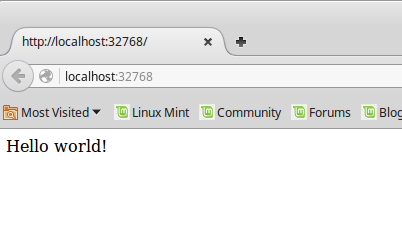
\includegraphics[angle=0,scale=0.75]{img/docker.png}
    \end{center}
    \caption{\em Działająca aplikacja webowa}
    \label{fig:webapp}
\end{figure}

\subsection{Tworzenie własnego obrazu}

Własny obraz można utworzyć na dwa sposoby:
\begin{itemize}
\item Poprzez aktualizację kontenera stworzonego na podstawie obrazu oraz zapisanie wprowadzonych zmian do obrazu
\item Za pomocą pliku \textit{Dockerfile}
\end{itemize}

 W pierwszym przypadku mamy utworzony kontener na podstawie obrazu i wprowadziliśmy do niego nowe dane, np. zainstalowaliśmy program. Nowy obraz tworzymy za pomocą polecenia:
\begin{lstlisting}[style=incode]
$ docker commit -m "Added program" -a "Author" bd625e9176a7 author/ubuntu:v2
\end{lstlisting}
gdzie
\begin{itemize}

\item \textit{docker commit} – zapisuje stn kontenera w postaci obrazu
\item \textit{-m} – flaga pozwalająca zapisać co zostało zmienione w obrazie
\item \textit{-a} – flaga informująca o autorze wprowadzonych zmian
\item \textit{bd625e9176a7} –  numer ID kontenera, na bazie którego tworzony jest nowy obraz
\item \textit{author/ubuntu:v2} – nazwa repozytorium oraz znacznik wersji utworzonego obrazu
\end{itemize}
Po wywołaniu tego polecenia moemy sprawdzić listę obrazów w lokalnym repozytorium:
\begin{lstlisting}[style=incode]
$ docker images
REPOSITORY          	TAG                 IMAGE ID            	     CREATED             	
SIZE
author/ubuntu       	   v2                  adbc62b82a11        19 seconds ago      	
725.1 MB
ubuntu         		  latest              b72889fa879c        11 days ago             	
188 MB
training/webapp   	  latest              6fae60ef3446        11 months ago     	  
348.8 MB 
\end{lstlisting}


Tworzenie obrazu z pliku \textit{Dockerfile} przebiega następująco. Najpierw tworzymy katalog na nasz plik, a w nim plik \textit{Dockerfile}:
\begin{lstlisting}[style=incode]
$ mkdir dockerbuild
$ cd dockerbuild/
$ touch Dockerfile
\end{lstlisting}
Zawartość pliku może wyglądać następująco:
\begin{lstlisting}[style=incode]
FROM ubuntu:14.04
MAINTAINER Author <author@example.com>
RUN apt-get update 
RUN apt-get install build-essential 
RUN apt-get install qt5-default
\end{lstlisting}
Plik \textit{Dockerfile} składa się z instrukcji, których nzwy pisane są wielkimi literami poprzedzających polecenia: \textit{INSTRUKCJA polecenie}. Wyjaśnienie instrukcji wykorzystanych w powyższym pliku:
\begin{itemize}

\item \textit{FROM ubuntu:14.04} – ta komenda mówi o tym, że obraz bazuje na obrazie systemu ubuntu wersji 14.04
\item \textit{MAINTAINER Author <author@example.com>} - wskazanie autora obrazu
\item \textit{RUN ...} - instrukcja RUN nakazuje wykonać w kontenerze dane polecenia
\end{itemize}
Następnie budujemy obraz na podstawie pliku \textit{Dockerfile} (przy wywołaniu tej komendy musimy znajdować się w katalogu, w którym jest nasz plik \textit{Dockerfile}):
\begin{lstlisting}[style=incode]
$ docker build -t author/ubuntu:v2 .
\end{lstlisting}


\subsection{Korzystanie z Docker Hub}

Utworzony obraz może zostac udostępniony w repozytorium Docker Hub, a następnie pobrany przez członków naszego zespołu. W tym celu należy się zalogować na swoje konto Docker Hub za pomoc klienta dockera:
\begin{lstlisting}[style=incode]
$ docker login
\end{lstlisting}
Po podaniu danych logowania możemy udostępnić obraz:
\begin{lstlisting}[style=incode]
$ docker push author/ubuntu:v2
\end{lstlisting}
Następnie może on zostać pobrany przez innch użytkowników:
\begin{lstlisting}[style=incode]
$ docker pull author/ubuntu:v2
\end{lstlisting}